\documentclass[conference]{IEEEtran}
% Short paper (progress report). Build: pdflatex main; bibtex main; pdflatex main; pdflatex main
% All numbers, tables and plots come from analysis/make_results.py run on the experiment database.
\usepackage[T1]{fontenc}
\usepackage{cite}
\usepackage{amsmath,amssymb}
\usepackage{graphicx}
\usepackage{booktabs}
\usepackage{xcolor}
\usepackage{tikz}
\usetikzlibrary{arrows.meta,positioning,fit,calc,backgrounds}
\usepackage{url}
\usepackage[hidelinks]{hyperref}
\usepackage{microtype}

\definecolor{cUrdu}{HTML}{009E73}
\definecolor{cRoman}{HTML}{D55E00}
\definecolor{cMixed}{HTML}{CC79A7}
\definecolor{cEng}{HTML}{0072B2}
\definecolor{cInk}{HTML}{333333}
\definecolor{cBox}{HTML}{F4F6F8}

\newcommand{\rom}[1]{\textit{#1}}  % Roman-Urdu text

\begin{document}

\title{Is the AI Judge Fair to Roman Urdu?\\ Measuring Script Bias in LLM-as-a-Judge}

\author{\IEEEauthorblockN{Syed Sheraz Anjum (25240017),\; Saif ur Rehman (24280071),\; Hussnain Ali Murtaza (25280069),\\
Junaid Tariq (25280044),\; Mukhammad Khasnen (25280090)}
\IEEEauthorblockA{2601 SSE Responsible AI Engineering (AI 630 S1-Lecture), Group 10 \\
Lahore University of Management Sciences (LUMS), Lahore, Pakistan}}

\maketitle

\begin{abstract}
Large language models (LLMs) are increasingly used as \emph{judges} that grade answers and rank model outputs.
Many of Urdu's roughly 230 million speakers type Urdu in Latin letters (\emph{Roman Urdu}) and freely mix in English
words, yet it is unknown whether LLM judges grade such text as fairly as standard Urdu script. We audit this with a
controlled perturb-and-compare design: 300 reading-comprehension items from Belebele are presented in four versions
that differ only in written form (Urdu script, Roman Urdu, Urdu--English code-mixed, English), and nine open and
commercial LLM judges from three companies at three size tiers score, compare and answer them, giving 191{,}760
judgements. Every judge that passes a screening gate scores the \emph{same correct answer} $0.55$--$1.26$ points lower
(on a 1--10 scale) in Roman Urdu than in Urdu script, and $0.59$--$1.30$ lower when code-mixed; English is scored higher.
The penalty replicates, persists among items the judge demonstrably understood in both scripts, and does not shrink
with model size even though larger judges discriminate correct from wrong answers better. Converting Roman Urdu to Urdu
script before judging is the most effective mitigation tested; an ``ignore spelling'' rubric mainly makes judges more
lenient. We describe the open evaluation platform built for the study, the challenges met, and the remaining work:
bilingual human validation, a spelling-variation study, and familiarity analysis.
\end{abstract}

\begin{IEEEkeywords}
LLM-as-a-judge, fairness, script bias, Roman Urdu, code-mixing, evaluation
\end{IEEEkeywords}

% =====================================================================
\section{Introduction}
LLM-as-a-judge has become a standard way to evaluate open-ended outputs at scale: it grades answers, ranks chatbot
replies and supplies preference signals for reward models \cite{zheng2023judging}. Its convenience rests on an
assumption that the judge scores \emph{content}, not \emph{presentation}. A growing literature shows the assumption is
fragile: judges favour their own generations \cite{panickssery2024llm}, prefer text they find familiar
\cite{wataoka2024self}, and react to a dozen kinds of irrelevant perturbation \cite{ye2025justice}.

Urdu raises a case that this literature has not isolated. The same language is written in two scripts: the
Perso-Arabic \emph{Urdu script} (\raisebox{-0.3ex}{
\includegraphics[height=1.9ex]{figures/urdu_example.pdf}}, ``five villages'') and \emph{Roman Urdu}
(\rom{paanch dehaat}), the Latin-letter form that dominates texting and social media. Speakers also code-mix
(\rom{paanch villages}). Roman Urdu has no standard orthography \cite{khan2022clustering}, so each spelling is rare in
training data. If a judge scores a correct Roman Urdu answer lower than the identical answer in Urdu script, then every
leaderboard, grading tool and reward model built on that judge quietly penalises the way millions of people actually
write---an allocational harm of the kind responsible-AI practice is meant to catch.

\textbf{Problem statement.} \emph{Holding content fixed, does the script an answer is written in---Urdu script, Roman
Urdu, Urdu--English code-mixed, or English---change how an LLM judge scores, compares and understands it, and can simple
interventions remove the effect?} We answer three sub-questions: (RQ1) Is there a score or preference gap? (RQ2) Is it
explained by comprehension failure, or does it persist when the judge understands the text? (RQ3) Does it shrink with
model scale or with mitigations (rubric instruction, transliteration, judge panel)?

\textbf{Contributions so far.} (i) A controlled four-version Urdu dataset in which only the written form varies;
(ii) an open, reproducible evaluation platform with full call provenance; (iii) a nine-judge, four-round audit showing
a consistent and replicated penalty for Roman and code-mixed Urdu; (iv) a first comparison of mitigations.

% =====================================================================
\section{Related Work}
\textbf{Bias in LLM judges.} CALM \cite{ye2025justice} quantifies twelve judge biases by perturbing inputs and checking
whether the verdict changes; we adopt this perturb-and-compare logic but vary a factor CALM does not isolate: the script
of one language. Self-preference \cite{panickssery2024llm} and familiarity effects \cite{wataoka2024self}, where lower
perplexity text receives higher scores, suggest a mechanism for script bias that we treat as a hypothesis, not an
established cause. MT-Bench established the paradigm and its position bias \cite{zheng2023judging}, which motivates
our order-balanced pairwise design.

\textbf{Multilingual judging.} Fu and Liu report low inter-judge agreement across 25 languages, worst for low-resource
ones, and that scale does not fix it \cite{fu2025reliable}; Zhou et al.\ find that equivalent content receives
different scores across languages \cite{zhou2026lower}; MM-Eval \cite{son2026mmeval} and the CIA suite
\cite{doddapaneni2025cross} benchmark multilingual evaluators, and Hada et al.\ call for calibration against
native-speaker judgements \cite{hada2024large}. All compare \emph{languages}; none compares two scripts of the same
language with the content held fixed.

\textbf{Romanization and Urdu.} Evidence on romanized input is mixed: native-script versus romanized messages change
LLM triage accuracy for Indian languages \cite{khullar2026script}, whereas U-MIRAGE reports \emph{better} results in
Roman Urdu than Urdu script for medical QA \cite{faheem2026umirage}, so we test two-sided. RomanSetu
\cite{husain2024romansetu} and RomanLens \cite{saji2025romanlens} show romanization interacts with models' internal
representations, and Jamil and Rafi study Roman Urdu inputs as a \emph{safety} failure mode \cite{jamil2026code};
none measures evaluator fairness.

\textbf{Dialect and code-mixing.} Dialect lowers LLM-judge consistency in toxicity detection \cite{faisal2025dialectal}
and triggers covertly biased decisions about people \cite{hofmann2024ai}. CodeMixBench \cite{yang2025codemixbench},
Lost in the Mix \cite{mohamed2025lost} and Code Mixologist \cite{gupta2026code} study understanding and building
code-mixed models; UrBLiMP measures Urdu linguistic competence \cite{adeeba2026urblimp}. We build on their
noun-switching view of code-mixing \cite{mohamed2025lost} and on the point that comprehension must be measured before
a score difference is called bias.

\textbf{Gap.} No prior work tests whether an LLM judge grades the \emph{same} Urdu answer differently when only its
script changes, separates that from comprehension, and tests mitigations. That intersection is our focus.

% =====================================================================
\begin{figure*}[t]
\centering
\resizebox{\textwidth}{!}{%
\begin{tikzpicture}[
  font=\footnotesize, >={Stealth[length=2.2mm]},
  stage/.style={draw=cInk!45, rounded corners=3pt, fill=cBox, inner sep=4pt, align=left, anchor=north west},
  head/.style={font=\footnotesize\bfseries, anchor=south west, inner sep=1pt},
  ver/.style={rounded corners=2pt, inner sep=2.5pt, text width=2.95cm, align=left, font=\scriptsize, text=white},
  arr/.style={->, thick, cInk!70}]
% Stage 1
\node[stage, text width=2.7cm, minimum height=3.35cm] (s1) at (0,0) {%
  \textbf{Belebele item}\\[2pt]
  Passage ($\approx$100 words)\\ Question\\ 4 answer options\\[3pt]
  300 items (seed 13)\\ $\rightarrow$ correct option\\ $\rightarrow$ one wrong option};
\node[head] at (s1.north west) {\textcolor{cInk}{\textsf{1} Data}};
% Stage 2: four versions
\node[stage, text width=3.25cm, minimum height=3.35cm] (s2) at (3.35,0) {};
\node[anchor=north west, inner sep=0pt] at ($(s2.north west)+(0.14,-0.14)$) {\textbf{Same answer, four scripts}};
\node[head] at (s2.north west) {\textcolor{cInk}{\textsf{2} Versions}};
\node[ver, fill=cUrdu, anchor=north] (v1) at ($(s2.north)+(0,-0.55)$) {Urdu script\hfill\raisebox{-0.25ex}{\colorbox{white}{
\includegraphics[height=1.55ex]{figures/urdu_example.pdf}}}};
\node[ver, fill=cRoman, below=2.5pt of v1] (v2) {Roman Urdu\hfill \rom{paanch dehaat}};
\node[ver, fill=cMixed, below=2.5pt of v2] (v3) {Code-mixed\hfill \rom{paanch villages}};
\node[ver, fill=cEng, below=2.5pt of v3] (v4) {English\hfill Five villages};
\node[font=\scriptsize, align=left, text width=3.1cm, below=3pt of v4, text=cInk] {Belebele's own: \rom{Paanch gaon}\\ \textcolor{cRoman}{reworded $\Rightarrow$ not used}};
% Stage 3: judges, a company x size grid
\node[stage, text width=3.6cm, minimum height=3.35cm] (s3) at (7.25,0) {};
\node[anchor=north west, inner sep=0pt] at ($(s3.north west)+(0.14,-0.14)$) {\textbf{9 judges, 3 companies}};
\node[head] at (s3.north west) {\textcolor{cInk}{\textsf{3} Judges}};
\foreach \x/\fam in {8.3/Alibaba, 9.4/Meta, 10.5/Google}
  \node[font=\scriptsize\bfseries, text=cInk] at (\x,-0.78) {\fam};
\foreach \y/\tier in {-1.2/S, -1.72/M, -2.24/L}
  \node[font=\scriptsize\bfseries, text=cInk] at (7.6,\y) {\tier};
\foreach \x/\y/\m in {8.3/-1.2/Qwen3.5 9B, 9.4/-1.2/Llama 3.1 8B, 10.5/-1.2/Gemma 3 12B,
                      8.3/-1.72/Qwen3 32B, 9.4/-1.72/Llama 3.3 70B, 10.5/-1.72/Gemma 3 27B,
                      8.3/-2.24/Qwen3 235B, 9.4/-2.24/Llama 4 Maverick, 10.5/-2.24/Gemini 2.5 Flash}
  \node[draw=cInk!30, fill=white, rounded corners=1.5pt, font=\tiny, align=center, text width=0.92cm,
        minimum height=0.44cm, inner sep=1pt] at (\x,\y) {\m};
\node[anchor=north west, font=\scriptsize, text=cInk, align=left, text width=3.5cm] at (7.4,-2.56)
  {temperature 0 $\cdot$ reasoning off\\ short replies $\cdot$ every call logged};
% Stage 4: tasks
\node[stage, text width=3.15cm, minimum height=3.35cm] (s4) at (11.5,0) {%
  \textbf{Tasks}\\[1pt]
  \textbf{Screening}: AUC $>0.7$?\\
  \textbf{Comprehension}: pick option\\
  \textbf{Pointwise}: score 1--10\\
  \textbf{Pairwise}: A / B / TIE,\\ \quad both orders\\
  \textbf{Repeats}: 50 items $\times$3\\[2pt]
  \textbf{Mitigations}: rubric line;\\ transliterate to Urdu; panel};
\node[head] at (s4.north west) {\textcolor{cInk}{\textsf{4} Experiments}};
% Stage 5: metrics
\node[stage, text width=2.75cm, minimum height=3.35cm] (s5) at (15.3,0) {%
  \textbf{Rule-based parsing}\\ (no LLM reads replies)\\[3pt]
  \textbf{Metrics} vs.\ Urdu script\\
  score gap (paired)\\ AUC, acceptance $\geq7$\\ win rate (fair $=50\%$)\\ accuracy, consistency\\[2pt]
  bootstrap 95\% CI\\ ($B{=}1000$)};
\node[head] at (s5.north west) {\textcolor{cInk}{\textsf{5} Analysis}};
\draw[arr] (s1.east |- 0,-1.65) -- (s2.west |- 0,-1.65);
\draw[arr] (s2.east |- 0,-1.65) -- (s3.west |- 0,-1.65);
\draw[arr] (s3.east |- 0,-1.65) -- (s4.west |- 0,-1.65);
\draw[arr] (s4.east |- 0,-1.65) -- (s5.west |- 0,-1.65);
\end{tikzpicture}}
\caption{Study design. Each Belebele item is rendered in four versions that differ only in written form; the passage
and question are always shown in the same script as the answer. Nine judges (S/M/L = small, medium, large) run five
experiment types and three mitigations; replies are parsed by deterministic code and compared against the Urdu-script
reference.}
\label{fig:pipeline}
\end{figure*}

% =====================================================================
\section{Dataset}
\label{sec:data}
\textbf{Source.} Belebele \cite{bandarkar2024belebele} provides the same multiple-choice reading-comprehension items
(passage, question, four options) in 122 language variants, including Urdu in Arabic script (\texttt{urd\_Arab}),
romanized Urdu (\texttt{urd\_Latn}) and English (\texttt{eng\_Latn}). We join the three variants on passage link and
question number and draw 300 items with a fixed seed (13). For each item we keep the correct option and one wrong option
chosen deterministically from the seed, so every judge sees the same answer pairs. Urdu passages average 99.9 words and
answers 5.3 words (English: 78.9 and 4.2).

\textbf{Why we generated our own Roman Urdu.} A pilot showed that Belebele's romanized options are frequently
\emph{reworded} rather than transliterated (Fig.~\ref{fig:pipeline}: \rom{dehaat} $\rightarrow$ \rom{gaon}). Across all
1{,}200 options, 590 (49.2\%) of Belebele's Roman Urdu options differ in word count from the Urdu-script option, which
would confound \emph{script} with \emph{wording}. We therefore produced word-by-word transliterations of all 1{,}200
options with Claude Opus~5.5 (high reasoning effort) under written rules: transliterate, never translate (\rom{seb},
never \rom{apple}); common Pakistani spellings; standard spelling for foreign names. Only 117 (9.8\%) of our
transliterations differ in word count, almost all by one word because izafat compounds are hyphenated
(\rom{sehat-e-aama}).

\textbf{Code-mixed version.} Following the noun-switching approach of \cite{mohamed2025lost}, the same model rewrote
each option in Roman Urdu with Urdu grammar, verbs and function words kept and selected nouns switched to English
(\rom{paanch villages}). All 300 items have a code-mixed version.

\textbf{Preprocessing and checks.} Generated options were validated automatically (four non-empty options per item, no
Urdu script remaining) and stored with the generator name and an ``auto-approved'' label; no human review has been done
yet (Sec.~\ref{sec:remaining}). For the Roman and code-mixed versions, the passage and question are Belebele's
\texttt{urd\_Latn} text. The derived data is released under Belebele's CC BY-SA 4.0 licence.

% =====================================================================
\section{Methodology}
\label{sec:method}
\textbf{Judges.} Nine judges from three companies at three size tiers (Fig.~\ref{fig:pipeline}): Alibaba's Qwen, Meta's
Llama and Google's Gemma/Gemini. All are queried through OpenRouter at temperature~0 with reasoning disabled and an
8-token reply limit (one exception: Llama~4 Maverick's pairwise calls, Sec.~\ref{sec:impl}); the requested and served
model, provider, tokens, cost and timestamp of every call are recorded.

\textbf{Experiments.} (1)~\emph{Screening gate}: on 20 items in Urdu script and English, a judge must separate correct
from wrong answers with AUC $>0.7$ in both; judges that fail are flagged because their bias estimates would be noise.
(2)~\emph{Comprehension}: the judge answers the multiple-choice question itself in each version. (3)~\emph{Pointwise}:
``Rate how correct and helpful this answer is from 1 to 10'' for the correct and the wrong answer in all four versions
(2{,}400 calls per judge). (4)~\emph{Pairwise}: the same answer in a non-reference version and in Urdu script, side by
side; ``Which answer is better, A or B? Reply A, B or TIE.'' Each pair is shown in both orders to cancel position bias
(3{,}600 calls per judge); a fair judge says TIE. (5)~\emph{Repeats}: a 50-item subset is scored three times to separate
bias from randomness.

\textbf{Mitigations.} (a)~\emph{Rubric}: the instruction ``Ignore script, spelling and formality; judge only correctness''
is prepended. (b)~\emph{Transliterate}: Roman and code-mixed passage, question and answer are converted to Urdu script by
a separate model (GPT-4o-mini) before judging. (c)~\emph{Panel}: the mean score of a round's three judges.

\textbf{Parsing and metrics.} Replies are parsed by deterministic rules (e.g.\ ``Score: 8/10''$\to$8, Urdu digits
accepted); unparseable replies and ties are counted separately, never as failures. With Urdu script as reference we
report, per judge and version: the \emph{severity gap}, the mean paired difference in score on the same correct answers
(negative = harsher); \emph{AUC}, the probability that a correct answer outscores a wrong one (Mann--Whitney, ties
$=\frac12$); \emph{acceptance}, the share scored $\geq7$, separately for correct and wrong answers; pairwise \emph{win
rate} (ties count half; fair $=50\%$); comprehension \emph{accuracy}; and the share of identical scores across repeats.
Uncertainty is a seeded percentile bootstrap with 1{,}000 resamples \cite{efron1993bootstrap}, paired over items for gaps.
To separate bias from comprehension (RQ2), we recompute the gap on items the judge answered \emph{correctly in both}
scripts in the comprehension task.

\textbf{Rounds.} Round~1 uses the three small judges; Round~2 repeats it with fresh (uncached) calls as a replication;
Rounds~3 and~4 use the medium and large judges.

% =====================================================================
\section{Implementation Progress}
\label{sec:impl}
\textbf{Platform.} We built a private web platform: a Python/FastAPI backend with SQLite storage, a Next.js frontend
(Findings, Results, Trends and a ``Test yourself'' page where a user types or speaks a question and sees every judge
score it in each script), deployed with Docker Compose behind a TLS proxy on an AWS EC2 instance. Runs are created from
the UI or from driver scripts and are idempotent: each call is cached under a hash of (model, prompt, parameters, repeat
index), so interrupted runs resume and re-analysis never pays twice. The replication round uses a separate repeat-index
range to force fresh calls. A hard budget cap refuses paid calls beyond US\$30. The test suite (pytest and Vitest) runs
end-to-end against offline mock judges.

\textbf{Completed.} All four rounds finished, plus one corrective re-run: 33 runs, 191{,}760 recorded judgements,
132{,}671 unique API calls served by 20 inference providers, for a total cost of US\$9.49. Every table and figure in this paper is regenerated from the
database by a single script.

\textbf{Challenges and technical decisions.}
\label{sec:challenges}
\emph{(i) Dataset wording drift}: Belebele's Roman Urdu is often reworded (Sec.~\ref{sec:data}), so we generated our own
transliterations. \emph{(ii) ``Thinking'' models}: Gemini~3.x and Qwen~3.7~Max force reasoning or were heavily rate
limited on the only provider, so Gemini~2.5~Flash and Qwen3-235B represent the large tier. \emph{(iii) Truncated replies}:
with an 8-token limit, Llama~4 Maverick began 86\% of its \emph{pairwise} replies with step-by-step reasoning
(``\#\# Step 1: Understand the task'') and was cut off, leaving its first pairwise run inconclusive (its pointwise and
comprehension replies parse normally). We re-ran its 3{,}600 pairwise calls with a 1{,}024-token limit for that task
only (mean reply 432 tokens; US\$1.88) and extended the deterministic parser to read a reasoned reply's \emph{final}
verdict (an explicit marker such as ``The final answer is: TIE'' or a boxed or bold letter, else a verdict phrase in
the last sentence such as ``Therefore, it's a tie''; anything ambiguous stays unreadable). Unreadable replies fell from 86\% to 0.4\%, and re-parsing the stored
replies of the four earlier pairwise runs changed none of their 43{,}200 results. Note that Maverick
therefore reasons before its pairwise verdict, unlike the other judges. \emph{(iv) Provider variance}: one
provider's copy of Qwen3-235B echoed prompts or returned broken text, so per-judge provider routing was added.
\emph{(v) Non-determinism}: even at temperature~0, only 32--98\% of repeated scores are identical, depending on judge and script; we therefore read only
300-item averages. \emph{(vi) Gate noise}: Qwen~3.5~9B passed screening in Round~1 (AUC 0.76) but narrowly failed in
Round~2 (0.69).

% =====================================================================
\section{Preliminary Results}
\label{sec:results}
\begin{table*}[t]
\centering
\caption{Main results. Score gap = mean score of the \emph{same correct answer} minus its Urdu-script score (1--10 scale; \textbf{bold}: paired-bootstrap 95\% CI excludes 0). Win = Roman-Urdu version preferred over the Urdu-script version head-to-head (ties count half; fair $=50\%$; \textbf{bold}: CI excludes 50\%). Acc.\ = comprehension accuracy; AUC = correct-vs-wrong separation; Acc.\,wrong = wrong answers scored $\geq 7$. $^\dagger$Failed the screening gate (AUC $\leq 0.7$). $^\ddagger$Pairwise re-run with a 1{,}024-token reply limit (Sec.~\ref{sec:challenges}).}
\label{tab:main}
\small
\setlength{\tabcolsep}{4pt}
\begin{tabular}{@{}ll rrr r rrr rr rr@{}}
\toprule
 & & \multicolumn{3}{c}{Score gap vs.\ Urdu script} & Win & \multicolumn{3}{c}{Acc.\ (\%)} & \multicolumn{2}{c}{AUC} & \multicolumn{2}{c}{Acc.\,wrong (\%)} \\
\cmidrule(lr){3-5}\cmidrule(lr){6-6}\cmidrule(lr){7-9}\cmidrule(lr){10-11}\cmidrule(lr){12-13}
Round & Judge & Roman & Mixed & English & Roman & Urdu & Roman & Eng. & Urdu & Roman & Urdu & Roman \\
\midrule
Small & Qwen 3.5 9B & \textbf{$-$0.81} & \textbf{$-$0.91} & +0.34 & \textbf{14} & 76 & 57 & 92 & 0.68 & 0.60 & 38 & 41 \\
 & Llama 3.1 8B$^\dagger$ & $-$0.12 & \textbf{$-$0.31} & +0.21 & \textbf{40} & 48 & 33 & 69 & 0.57 & 0.54 & 78 & 71 \\
 & Gemma 3 12B & \textbf{$-$0.59} & \textbf{$-$0.86} & \textbf{+0.57} & \textbf{40} & 82 & 67 & 91 & 0.74 & 0.64 & 39 & 51 \\
 & \emph{Panel (mean)} & \textbf{$-$0.51} & \textbf{$-$0.69} & \textbf{+0.38} &  &  &  &  & 0.75 & 0.64 &  &  \\
\midrule
Replication & Qwen 3.5 9B$^\dagger$ & \textbf{$-$1.13} & \textbf{$-$1.19} & \textbf{+0.41} & \textbf{8} & 79 & 59 & 93 & 0.67 & 0.60 & 42 & 44 \\
 & Llama 3.1 8B$^\dagger$ & $-$0.29 & \textbf{$-$0.46} & +0.13 & \textbf{34} & 49 & 36 & 73 & 0.56 & 0.51 & 78 & 74 \\
 & Gemma 3 12B & \textbf{$-$0.82} & \textbf{$-$0.91} & \textbf{+0.48} & \textbf{39} & 83 & 69 & 91 & 0.73 & 0.64 & 41 & 49 \\
 & \emph{Panel (mean)} & \textbf{$-$0.75} & \textbf{$-$0.86} & \textbf{+0.35} &  &  &  &  & 0.73 & 0.64 &  &  \\
\midrule
Medium & Qwen3 32B & \textbf{$-$0.82} & \textbf{$-$0.97} & \textbf{+1.38} & \textbf{25} & 83 & 66 & 94 & 0.76 & 0.67 & 31 & 38 \\
 & Llama 3.3 70B & \textbf{$-$0.55} & \textbf{$-$0.59} & \textbf{+0.43} & \textbf{17} & 88 & 73 & 94 & 0.81 & 0.66 & 34 & 57 \\
 & Gemma 3 27B & \textbf{$-$0.92} & \textbf{$-$0.99} & +0.08 & \textbf{37} & 86 & 71 & 93 & 0.74 & 0.67 & 43 & 54 \\
 & \emph{Panel (mean)} & \textbf{$-$0.76} & \textbf{$-$0.85} & \textbf{+0.63} &  &  &  &  & 0.82 & 0.70 &  &  \\
\midrule
Large & Qwen3 235B & \textbf{$-$1.26} & \textbf{$-$1.30} & \textbf{+1.29} & \textbf{24} & 90 & 76 & 95 & 0.81 & 0.68 & 14 & 20 \\
 & Llama 4 Maverick & \textbf{$-$0.71} & \textbf{$-$0.85} & \textbf{+0.87} & \textbf{49}$^\ddagger$ & 85 & 66 & 93 & 0.81 & 0.66 & 25 & 40 \\
 & Gemini 2.5 Flash & \textbf{$-$0.78} & \textbf{$-$0.96} & \textbf{+0.48} & \textbf{48} & 91 & 86 & 96 & 0.87 & 0.81 & 14 & 16 \\
 & \emph{Panel (mean)} & \textbf{$-$0.92} & \textbf{$-$1.04} & \textbf{+0.88} &  &  &  &  & 0.89 & 0.80 &  &  \\
\bottomrule
\end{tabular}
\end{table*}

\begin{figure*}[t]
\centering
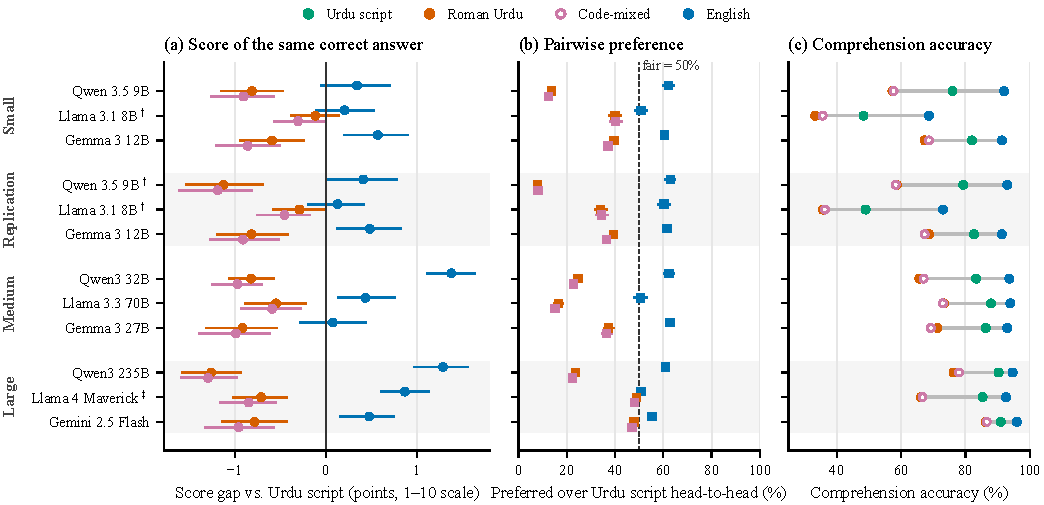
\includegraphics[width=\textwidth]{figures/overview.pdf}
\caption{Three views of script bias for every judge (bars: 95\% bootstrap CI). (a)~Score of the same correct answer
relative to Urdu script: Roman Urdu and code-mixed are consistently penalised, English is favoured. (b)~Head-to-head
preference against the Urdu-script version (50\% = fair); $^\ddagger$Llama~4 Maverick from its pairwise re-run.
(c)~Comprehension accuracy: judges understand Roman Urdu about 15 points worse than Urdu script, except
Gemini~2.5~Flash. $^\dagger$Failed screening.}
\label{fig:overview}
\end{figure*}

\textbf{RQ1: a consistent penalty.} Table~\ref{tab:main} and Fig.~\ref{fig:overview}a show that every judge that passes
screening scores the same correct answer lower in Roman Urdu ($-0.55$ to $-1.26$) and code-mixed text ($-0.59$ to
$-1.30$) than in Urdu script, with every confidence interval excluding zero; English is scored higher (up to $+1.38$).
The ordering English $>$ Urdu script $>$ Roman Urdu $\approx$ code-mixed holds for all three companies and all sizes.
Head-to-head (Fig.~\ref{fig:overview}b), most judges prefer the Urdu-script version: the Qwen judges pick Roman Urdu in
only 8--25\% of comparisons and Llama~3.3~70B in 17\%. Gemini~2.5~Flash and (re-run, reasoning) Llama~4 Maverick
come closest to fair: both answer TIE in 95\% of Roman-vs-Urdu comparisons (win rates 48\% and 49\%). Yet even they
lean the same way when they do decide: Gemini prefers the Urdu-script version 54 times to 1 (code-mixed: 71 to 0) and
Maverick 43 to 18 (71 to 22), so both win rates remain significantly below 50\%. The panel of each round's judges inherits the bias ($-0.51$, $-0.75$, $-0.76$, $-0.92$ for
the four rounds; all significant), because the judges lean the same way.

\textbf{Mistakes slip through.} Wrong answers are accepted (scored $\geq7$) more often in Roman Urdu than in Urdu script
for every passing judge, e.g.\ Llama~3.3~70B 57\% vs.\ 34\%, Llama~4 Maverick 40\% vs.\ 25\%; error detection drops
accordingly (AUC 0.81 $\to$ 0.66 for both). Roman Urdu answers are thus penalised when right \emph{and} under-scrutinised
when wrong.

\textbf{Replication.} Round~2 reproduces Round~1 with fresh calls, with somewhat larger gaps (Qwen~3.5~9B $-0.81\to-1.13$;
Gemma~3~12B $-0.59\to-0.82$) and nearly identical comprehension and AUC.

\textbf{RQ2: not only comprehension.} Judges do understand Roman Urdu less well (Fig.~\ref{fig:overview}c; e.g.\
Qwen3-235B 90\% vs.\ 76\%), but restricting to items the judge answered correctly \emph{in both} scripts leaves the
penalty intact: $-0.57$ (Gemini~2.5~Flash, $n{=}252$) to $-1.35$ (Qwen3-235B, $n{=}220$), every interval excluding
zero. A judge that demonstrably understood the answer still scored it lower in Latin script.

\begin{figure}[t]
\centering
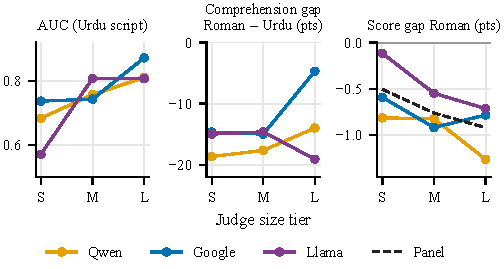
\includegraphics[width=\columnwidth]{figures/scale.pdf}
\caption{Scale makes judges better but not fairer. From small (S) to large (L) judges, error detection in Urdu script
(AUC) rises in every family, the comprehension gap narrows clearly only for Google, and the Roman-Urdu score penalty does not
shrink; the panel's penalty grows.}
\label{fig:scale}
\end{figure}

\textbf{RQ3a: scale.} Fig.~\ref{fig:scale} contrasts quality and fairness across tiers. Larger judges discriminate
better (Urdu-script AUC 0.57--0.74 $\to$ 0.81--0.87) and are more consistent (identical scores on repeat up to 96--98\%
for Gemini~2.5~Flash), yet the Roman score penalty does not shrink: the largest gap in the study is from the largest
judge (Qwen3-235B, $-1.26$), and the large-round panel penalty ($-0.92$) is the largest of all rounds.

\begin{figure}[t]
\centering
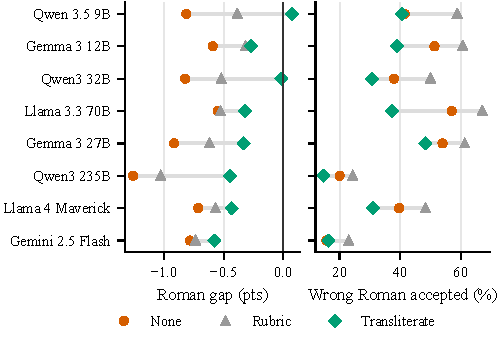
\includegraphics[width=\columnwidth]{figures/mitigation.pdf}
\caption{Mitigations (judges that passed screening). Left: Roman-Urdu score gap; right: wrong Roman-Urdu answers
accepted. Transliterating to Urdu script first shrinks the gap most and lowers false acceptance; the rubric line
narrows the gap mainly by accepting more wrong answers.}
\label{fig:mitig}
\end{figure}

\textbf{RQ3b: mitigations.} Converting Roman and code-mixed text to Urdu script before judging (Fig.~\ref{fig:mitig})
leaves no significant gap for four of the five passing small and medium judges in Rounds~1 and~3 (e.g.\ Qwen3-32B
$-0.82\to-0.02$; Llama~3.3~70B keeps $-0.32$) and lowers wrong-answer acceptance (Llama~3.3~70B $57\%\to37\%$), but a
significant gap remains for Gemma~3~12B in the replication round ($-0.47$) and for all three large judges ($-0.43$ to
$-0.58$). The rubric line narrows the gap only partly (it remains significant for every medium and large judge) and
raises wrong-answer acceptance for every passing judge (e.g.\ Qwen~3.5~9B $41\%\to59\%$): it buys leniency, not fairness.

\textbf{Tokenization is not the whole story.} From uncached comprehension calls, Llama and Qwen3 tokenizers spend more
tokens on Urdu-script prompts ($\approx$480--500) than on Roman Urdu ($\approx$350), whereas Gemma's tokenizer is the
reverse (271 vs.\ 312). Yet all three families penalise Roman Urdu, so token length alone does not explain the effect.

% =====================================================================
\section{Remaining Work}
\label{sec:remaining}
\begin{enumerate}
\item \textbf{Human validation.} Bilingual raters will (a) check the fidelity of a random sample of 100 generated
Roman and code-mixed options, and (b) rate a subset of answers in each script, giving a human reference against which
to calibrate judge scores \cite{hada2024large}.
\item \textbf{Reasoning as a mitigation.} One of the two judges closest to fair head-to-head is the re-run Maverick,
which reasons before its pairwise verdict. We will test whether asking every judge to reason (or to first state whether the two answers say the
same thing) reduces the pointwise penalty, and repeat Maverick's pairwise test with a strict answer-only format to
separate the effect of reasoning from that of the model.
\item \textbf{Spelling-variation study.} Our transliterations use one consistent spelling, while real Roman Urdu varies
widely \cite{khan2022clustering}. We will score several realistic spellings of each answer to test whether
non-standard orthography drives the penalty.
\item \textbf{Familiarity analysis.} Our platform already computes per-character perplexity of every answer under an
open model; we will correlate it with per-item gaps to test the familiarity hypothesis \cite{wataoka2024self}.
\item \textbf{Remove the passage confound.} Roman and code-mixed prompts currently use Belebele's (partly reworded) Roman
Urdu passages; a condition with fully transliterated passages will isolate script effects end to end.
\item \textbf{Open-ended answers.} Extend from multiple-choice options to free-text, student-style answers, the
academic-marking setting that motivates the work.
\item \textbf{Statistics and reporting.} Mixed-effects models with item random effects and Holm correction across
judges; release of data, code and practitioner guidelines.
\end{enumerate}

% =====================================================================
\section{Conclusion}
Across nine judges, three companies, three sizes and a replication, LLM judges consistently score the same correct
answer lower when Urdu is written in Latin script, and catch fewer wrong Roman-Urdu answers. The penalty persists when
the judge understood the text and does not shrink with scale. Transliterating to Urdu script before judging is the
most effective mitigation we tested, while ``ignore spelling'' instructions mostly add leniency. Practitioners using
LLM judges for South Asian languages should report results per script and keep a human in the loop for Roman Urdu.

\bibliographystyle{IEEEtran}
\bibliography{refs}

\end{document}
